%% %% 版本作者:
%% %%   Wizen Zhang
%% %%   E-mail:wizen_zhang@163.com
%% %%   GitHub:https://github.com/WizenZhang/NMUProposal
%% %%=================================================================
%% %% <UTF-8>
%% %% 北方民族大学硕士学位论文开题报告书LaTeX模板--始于 2018/10/27
%% %% 请将以下文件与此LaTeX文件放在同一目录中.
%% %%-----------
%% %% NMUProposal.tex         : LaTeX模板运行入口(main)
%% %% NMUProposal.pdf         : PDF模板样例
%% %% nmu.cls                 : LaTeX宏模板文件
%% %% GBT7714-2005.bst        : 国标参考文献BibTeX样式文件2005(https://github.com/Haixing-Hu/GBT7714-2005-BibTeX-Style)
%% %% GBT7714-2015.bst        : 国标参考文献BibTeX样式文件2015(https://github.com/zepinglee/gbt7714-bibtex-style)
%% %% tex/*.tex               : LaTeX模板样例中的独立章节
%% %% figures/*               : LaTeX模板样例中的插图存放目录
%% %% ref.bib                 : LaTeX模板中的参考文献Bib文件
%% %% make.bat                : 生成NMUProposal.pdf
%% %% clean.bat               : 清理冗余文件
%% %%-----------
%% %% 请统一使用UTF-8编码.
%% %%=================================================================
%% %%LaTeX安装配置教程请参看:https://jingyan.baidu.com/article/b2c186c83c9b40c46ff6ff4f.html
%%LaTeX入门视频教程请参看:https://blog.csdn.net/so_geili/article/details/51702564
%=================================================================
\documentclass{nmu}% thesis template of UCAS
\usepackage{titlesec}   %设置页眉页脚的宏包
%=================================================================
% 插图路径设置,图片放在figures 文件夹下。一般来说论文的插图比较多,通常按章节存
% 放,因此可以在以下命令中在按章节添加存放图片的文件夹路径。如以下这个路径中 ./
% 代表当前NMUProposal.tex所在的目录,就是一般所说的当前文件夹;figures 文件夹就是子文件
% 夹,存放正文及附录中要用到的所有的图片,在figures 文件夹中的子文件夹就是存放各
% 个章节图片的文件夹,一般命名与相应章节的名字相同,如section_sample章节用到的图片全放在
% 了sample这个子文件夹下。
\graphicspath{{./figures/sample/},{./figures/}}
\bibliographystyle{GBT7714-2015}
%%=================================================================
\author{学生姓名}                                 % 报告人

\major{计算机系统结构}                             % 专业

\field{开题报告\LaTeX{}编程研究}                   % 研究方向

% 导师 (专硕增加企业导师),第一参数为校内导师内容,第二个参数为企业导师内容
% 若无增加企业导师,需删除nmu.cls中 "& \NMUunderline[256pt]{\NMU@value@secadvisor} \\" 对应的一行	
\advisor{校内导师~~教授}{企业导师~~高级工程师}      

% 论文标题, 因title一般都很长需要两行,第一参数为第一行内容,第二个参数为第二行内容
% 若论文标题只有一行,需删除nmu.cls中 "& \NMUunderline[256pt]{\NMU@value@sectitle} \\" 对应的一行
\nmutitle{北方民族大学硕士学位论文}{开题报告书\LaTeX{} 模板}

\institute{计算机科学与工程学院}                   % 学院

\chinesedate{2018~年~10~月~24日}                  % 开题日期

\begin{document}
% 封皮
\maketitle
%%=================================================================
%% 添加正文内容
\pagenumbering{arabic}  %restart page numbers with arabic style

% 1.本课题的研究目的与意义
% 2.与选题相关的国内外研究状况及最新动态
% 3.本课题的基本内容
% 4.本课题的重点和难点
% 5.本课题实验设计及创新之处
% 6.可行性论证
% 7.论文提纲
% 8.调研进度安排
% 9.预期目标
% 10.与本课题相关的主要参考文献
%%%%% --------------------------------------------------------------------------------
%%
%%%%******************************* Main Content *************************************
%%
%%% ++++++++++++++++++++++++++++++++++++++++++++++++++++++++++++++++++++++++++++++++++
\begin{framedbox}
\section{本课题的研究目的与意义} 
\NMUtableline
\subsection{模板简介}
本模板为《北方民族大学硕士学位论文开题报告书\LaTeX{} 模板》,清单如表 \ref{tab:papercomponents} 所示,模板中大量内容为使用说明及例程,基本覆盖了内容和格式方面的要求,对于新手请仔细阅读,根据自身情况作出相应的修改,此模板的学习和使用也方便今后的学位论文\LaTeX{} 排版。

\begin{table}[h]
	\caption{开题报告书清单}
	\label{tab:papercomponents}
	\centering
	\begin{tabular}{cp{18\ccwd}p{3cm}}
		\toprule
		  {\songti\bfseries 装订顺序} & \multicolumn{1}{c} {\songti\bfseries 内容} & \multicolumn{1}{c} {\songti\bfseries 说明}  \\
		\midrule
		1 & 封面                               &  更改相应标签 \\        
		2 & 开题报告填写要求                    &              \\
		3 & 本课题的研究目的与意义              &              \\
		4 & 与选题相关的国内外研究状况及最新动态 &              \\
		5 & 本课题的重点和难点                  &              \\
		6 & 本课题的重点和难点                  &              \\
		7 & 本课题实验设计及创新之处            &               \\
		8 & 可行性论证	                      &               \\
		9 & 论文提纲                           & 更改相应表格  \\
		10& 调研进度安排                       &  更改相应时间  \\
		11& 预期目标                           &               \\
		12& 与本课题相关的主要参考文献          & ref.bib文件   \\
		13& 指导教师意见                       &               \\
		14& 研究生学位论文开题报告评议书        &               \\
		\bottomrule
	\end{tabular}
\end{table}

\subsection{友情链接}

《北方民族大学硕士学位论文开题报告书\LaTeX{} 模板》下载地址:

\href{https://github.com/WizenZhang/NMUProposal}{https://github.com/WizenZhang/NMUProposal}

Windows系统可以选择TexLive+TeXstudio的方式安装,配置教程请参看:

\href{https://jingyan.baidu.com/article/b2c186c83c9b40c46ff6ff4f.html}{https://jingyan.baidu.com/article/b2c186c83c9b40c46ff6ff4f.html}


\LaTeX{}入门视频教程请参看:

\href{https://blog.csdn.net/so_geili/article/details/51702564}{https://blog.csdn.net/so\_geili/article/details/51702564}

后续使用《北方民族大学学位论文\LaTeX{}模板》下载地址:

\href{https://github.com/WizenZhang/NMUThesis}{https://github.com/WizenZhang/NMUThesis}


\newpage
\subsection{模板使用目的}

Word 是 见什么就是什么,用户的精力集中在视觉效果。\LaTeX{} 是 想什么就写什么,用户的精力集中在结构和内容。\LaTeX{}相对于Word有何优势?体现在以下几点:

\begin{itemize}[topsep=0pt,partopsep=0pt,itemsep=0pt,parsep=0pt]
\item 方便的实现数学公式、图表、章节的自动编号和交叉引用,自动格式化文字段落,避免个别字符的格式错误。你只需要说这是标题、那是引用、这是插图,\LaTeX{} 就把他们放在应该放的地方,不用多操心位置、大小、字体等细节。很多学术期刊提供模版,进一步节省了作者{\bfseries \songti 调整格式}的时间。
\item 可以保存撰写过程的中间信息:修改时把打算删除的段落注释起来,后悔时取消注释即可,这个在Word里很难实现;还可以用注释记下相关的信息,如粗糙的灵感等等,以便进一步发展思路,在Word里用“注释”倒是可以实现,但正式发布的时候,还要一条条删除,麻烦!
\item 数学公式美观专业,输入非常便捷,只要知道怎么读,就知道怎么写。平时和别人用纯文字交流数学时,也会用 \LaTeX{} 代码。化学式,乐谱,各专业的冷门特殊符号,也都有很便捷的支持。	
\item 鼓励,甚至强制用户定义清晰的文章结构,有助于养成良好的论文写作习惯。结构命令易于理解和记忆,和日常英语会话几乎一致,并且可以方便地生成参考文献、脚注、目录、索引等。	
\end{itemize}

\subsection{模板使用意义}
就排版的专业程度上来说,Word 被甩得很远。用 Word 写论文,花大量时间纠结格式,还不一定能搞定。这样的专业性大大方便了作者和审稿、编辑关于格式的交流。大量专业书籍、期刊、甚至字典,是由 TeX 制作的。

\begin{itemize}
	\item 不会用\LaTeX{} $\rightarrow$ 无法编译 没有文档
	\item 不会用Word $\rightarrow$ 文档真难看 格式丑死了
	\item 会用Word $\rightarrow$  文档
	\item \LaTeX{} 用的好 $\rightarrow$  牛逼的文档
	\item Word 用的好 $\rightarrow$  牛逼的文档
\end{itemize}

\newpage 
\section{与选题相关的国内外研究状况及最新动态} 
\NMUtableline 

\begin{center}
	\zihao{4}关于封面研究方向填写规则
\end{center}

\subsection{专业硕士从以下四个方向选择一个}

\begin{enumerate}[label=\arabic*)]
	\item 信息系统设计与开发;
	\item 嵌入式技术及应用;
	\item 计算机图形学及图像处理技术;	
	\item 计算机网络与控制系统
\end{enumerate}

\subsection{计算机科学与技术 学硕从以下四个方向选择一个}

\begin{enumerate}[label=\arabic*)]
	\item 计算机图形图像处理与分析;
	\item 数据库与知识工程;
	\item 嵌入式系统与物联网技术研究;	
	\item 计算机网络与移动计算
\end{enumerate}

\subsection{软件工程 学硕从以下方向选择一个}

\begin{enumerate}[label=\arabic*)]
	\item 软件服务工程;
	\item 嵌入式技术及应用;
	\item 图像与信号处理;	
\end{enumerate}
 
\newpage  
\section{本课题的基本内容} 
\NMUtableline

\begin{itemize}
	\item[■] 注意事项
\end{itemize}

请将表 \ref{tab:tabu_file} 中文件清单放在同一目录中,打开“\verb|NMUProposal.tex|”文件并启动全运行,即可生成“\verb|NMUProposal.pdf|”示例文件。主题内容在“\verb|section1-10.tex|”中编写,如需换页请使用“\verb|\newpage|”命令,如需加线请使用\verb|\NMUtableline|命令(注意线和文字间的空行),具体编码实现请参看相应的示例。

\begin{longtable}{|c|>{\raggedright\arraybackslash}p{8cm}|}
	\caption{北方民族大学硕士学位论文开题报告书\LaTeX{} 模板清单表}\label{tab:tabu_file}
	\endfirsthead
	\caption{北方民族大学硕士学位论文开题报告书\LaTeX{} 模板清单表(续)}
	\endhead
	\hline 
	\rule[0ex]{0pt}{2.5ex} \verb|NMUProposal.tex| & $\triangleright$\LaTeX{}模板运行入口(main) \\ 
	\hline 
	\rule[0ex]{0pt}{2.5ex} \verb|NMUProposal.pdf| & $\triangleright$PDF模板样例\\
	\hline 
	\rule[0ex]{0pt}{2.5ex} \verb|nmu.cls |    & $\triangleright$ \LaTeX{}宏模板文件 \\
	\hline 
	\rule[0ex]{0pt}{2.5ex} \verb|GBT7714-2005.bst| & $\triangleright$ 国标参考文献BibTeX样式文件2005 \\
	\hline 
	\rule[0ex]{0pt}{2.5ex} \verb|GBT7714-2015.bst|  & $\triangleright$ 国标参考文献BibTeX样式文件2015 \\
	\hline  
	\rule[0ex]{0pt}{2.5ex} \verb|tex/*.tex| & $\triangleright$\LaTeX{}模板样例中的独立章节\\
	\hline 
	\rule[0ex]{0pt}{2.5ex} \verb|figures/*| & $\triangleright$\LaTeX{}模板样例中的插图存放目录\\
	\hline 
	\rule[0ex]{0pt}{2.5ex} \verb|ref.bib |    & $\triangleright$\LaTeX{}模板中的参考文献Bib文件\\
	\hline 
	\rule[0ex]{0pt}{2.5ex} \verb|make.bat|    &$\triangleright$生成NMUProposal.pdf\\
	\hline 
	\rule[0ex]{0pt}{2.5ex} \verb|clean.bat|  & $\triangleright$清理冗余文件\\
	\hline 
\end{longtable}

\begin{itemize}
	\item[$\triangleright$] 调整表格行间距可使用\verb|\rule[0ex]{0pt}{2.5ex}|或\verb|\def\arraystretch{1.5}|,具例参看表\ref{tab:tabu_file}和\ref{tab:schedule}格式;
	\item[$\triangleright$] 封面若无增加企业导师,需删除nmu.cls中:
	
	“\verb|\NMUunderline[256pt]{\NMU@value@secadvisor} \\”| 对应的一行;
	\item[$\triangleright$] 封面若论文标题只有一行,需删除nmu.cls中:
	
	“\verb|\NMUunderline[256pt]{\NMU@value@sectitle} \\”|对应的一行;
	\item[$\triangleright$] 若某文献标题中含有特定含义大写字母(“ISODATA”等,详见\cite{Li2017An}),应特别用第二重{}将其括起来才可使其正常表示;
	\item[$\triangleright$] \verb|\label{<text>}|中不能使用中文;
	\item[$\triangleright$] 浮动体与正文之间的距离是弹性的
\end{itemize}

\newpage
\section{本课题的重点和难点} 
\NMUtableline

\subsection{参考文献引用}

参考文献类型:专著[M],会议论文集[C],报纸文章[N],期刊文章[J],学位论文[D],报告[R],标准[S],专利[P],论文集中的析出文献[A]。测试一下上标引用\upcite{Le2016Multiple},引用\cite{Le2016Multiple,Kaya2015,tf2017},还有其它引用\upcite{Li2017An,Le2016Multiple,tf2017}.


\subsection{导入BibTeX参考文献库可通过百度学术或Zotero等(例:如图\ref{fig:3-1}、\ref{fig:3-2})}



\begin{figure}[tbh!]
	\centering
	\includegraphics[width=0.6\linewidth]{figures/sample/3-1}
	\caption{导入BibTeX参考文献库步骤一}
	\label{fig:3-1}
\end{figure}

\begin{figure}[tbh!]
	\centering
	\includegraphics[width=0.6\linewidth]{figures/sample/3-2}
	\caption{导入BibTeX参考文献库步骤二}
	\label{fig:3-2}
\end{figure}

\newpage
\section{本课题实验设计及创新之处} 
\NMUtableline

\subsection{表格、图片可使用TeXstudio向导插入(例:如图\ref{subfig:3a}、\ref{subfig:3b})}

\begin{figure}[htb!]
	\centering
	\begin{subfigure}[b]{.4\textwidth}
		\centering
		\includegraphics[width=0.7\linewidth]{3-3.png}
		\caption{TeXstudio向导}\label{subfig:3a}
	\end{subfigure}
	\begin{subfigure}[b]{.4\textwidth}
		\centering
		\includegraphics[width=\linewidth]{3-4.png}
		\caption{插入图片}\label{subfig:3b}
	\end{subfigure}
	\caption{使用TeXstudio向导插入图片}\label{fig:3}
\end{figure}

\subsection{\LaTeX{}中插入Visio图}

\begin{enumerate}[label=\arabic*)]
	\item Visio原图另存为PDF格式;
	\item 用Acrobat打开,文档 -- 剪裁页面 -- 删除白边距;
	\item 将pdf格式文件复制到figures文件夹,如nmu.cls中插入封皮标题文字\\ \verb|\includegraphics[scale=1.0]{proposal.pdf}|;	
	\item 或另存为eps格式;
	\item 将eps格式文件复制到figures文件夹
	\item 类似插入图片的方式将图插入
\end{enumerate}

\newpage
\section{可行性论证} 
\NMUtableline 

\subsection{算法环境}

模板中使用 \texttt{algorithm2e} 宏包实现算法 \ref{alg:partition},关于该宏包的具体用法请阅读宏包的官方文档。

\RestyleAlgo{boxruled}
\begin{algorithm}[!h]
	\caption{PARTITION$(A,p,r)$ (boxruled)}%算法标题
	\label{alg:partition}
	\KwData{this text}
	\KwResult{how to write algorithm with \LaTeX2e{} }
	\begin{algorithmic}[1]%一行一个标行号
		\STATE $i=p$
		\FOR{$j=p$ to $r$}
		\IF{$A[j]<=0$}
		\STATE $swap(A[i],A[j])$
		\STATE $i=i+1$
		\ENDIF
		\ENDFOR
	\end{algorithmic}
\end{algorithm}

\subsection{代码环境}

listings 是专用于代码排版的\LaTeX{}宏包,可对关键词、注释和字符串等使用不同的字体和颜色或颜色,也可以为代码添加边框、背景等风格。很多时候需要对文档中的代码进行解释,只有带有行号的代码才可以让解释更清晰,因为你只需要说第 x行代码有什么作用即可。如果没有行号,那对读者而言就太残忍了,他们不得不从你的文字叙述中得知行号信息,然后去一行一行的查到相应代码行。listings 宏包通过参数 numbers 来设定行号,该参数的值有两个,分别是 left 与right,表示行号显示在代码的左侧还是右侧。下面给出一份用于排版C语言程序代码样例如图 \ref{fig:code} 所示。
\begin{figure}[htb!]
	\centering
	\begin{lstlisting}[language={[ANSI]C}] 
	int main(int argc, char ** argv) 
	{ 
	/*格式化并输出结果到标准输出*/
	printf("`我爱TeXing`! \n"); 
	return 0; 
	} 
	\end{lstlisting} 
	\caption{C语言程序代码样例}
	\label{fig:code}
\end{figure}

\newpage
\subsection{流程图}

流程图是表达算法思想最为有效的图形工具。作为计算机专业的学生,我们经常需要在文档中使用流程图来描述算法。在 LaTeX 中使用流程图可以通过 TikZ 或 flowchart 宏包来实现,但从本质上来说 flowchart 宏包也是使用 TikZ 宏包来实现的。flowchart 定义的形状数量比较少,可能满足不了绘制复杂流程图的需要,直接使用TikZ强大的绘图功能来实现流程图的绘制如图 \ref{fig:chart} 所示。

\begin{figure}[htb!]
	\centering
	\begin{tikzpicture}[node distance=1.8cm]
	%定义流程图具体形状
	\node (start) [startstop] {Start};
	\node (in1) [io, below of=start] {Input};
	\node (pro1) [process, below of=in1] {Process 1};
	\node (dec1) [decision, below of=pro1, yshift=-0.5cm] {Decision 1};
	\node (dec2) [decision, below of=dec1, yshift=-1.5cm] {Decision 2};
	\node (pro2) [process, right of=dec1, xshift=3cm] {Process 2};
	\node (out1) [io, below of=dec2, yshift=-0.5cm] {Output};
	\node (stop) [startstop, below of=out1] {Stop};
	\coordinate (pointN) at (-3cm, -9.2cm);
	%连接具体形状
	\draw [arrow](start) -- (in1);
	\draw [arrow](in1) -- (pro1);
	\draw [arrow](pro1) -- (dec1);
	\draw [arrow](dec1) -- (dec2);
	\draw [arrow](dec1) -- (pro2);
	\draw [arrow](dec1) -- node[anchor=east] {Y} (dec2);
	\draw [arrow](dec1) -- node[anchor=south] {N} (pro2);
	\draw [arrow](pro2) |- (pro1);
	\draw [arrow](dec2) -- node[left] {Y} (out1);
	\draw (dec2) -- node[above] {N} (pointN);
	\draw [arrow](pointN) |- (pro1);
	\draw [arrow](out1) -- (stop);
	\end{tikzpicture}
	\caption{直接使用TikZ宏包绘制的流程图}
	\label{fig:chart}
\end{figure}

\newpage
\subsection{数学环境}

模板定义了一些正体(upright)的数学符号:
\begin{center}
	\begin{tabular}{rl}
		\toprule
		符号                 & 命令 \\
		\midrule
		常数$\eu$     & \verb|\eu| \\
		复数单位$\iu$ & \verb|\iu| \\
		微分符号$\diff$ & \verb|\diff| \\
		$\argmax$         & \verb|\argmax| \\
		$\argmin$         & \verb|\argmin| \\
		\bottomrule
	\end{tabular}
\end{center}

更多的例子:
\begin{equation}
\eu^{\iu\pi} + 1 = 0
\end{equation}
\begin{equation}
\frac{\diff^2u}{\diff t^2} = \int f(x) \diff x
\end{equation}
\begin{equation}
\argmin_x f(x)
\end{equation}

\subsection{定理、引理和证明}


	A sigmoid function is a mathematical function having a characteristic "S"-shaped curve or sigmoid curve. Often, sigmoid function refers to the special case of the logistic function shown in the first figure and defined by the formula:
	\begin{equation}
	sigmoid(x) = \frac{1}{1 + e^{-x}}
	\end{equation}
	
	\begin{figure}[htb]
		\centering
		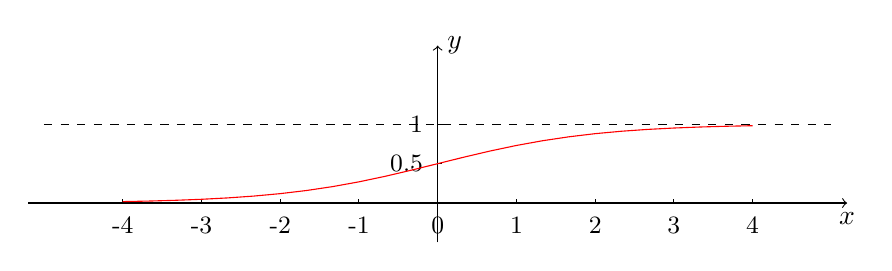
\begin{tikzpicture}
		\draw[->](-5.2,0)--(5.2,0)node[left,below]{$x$};
		\draw[->](0,-0.5)--(0,2)node[right]{$y$};
		\draw[dashed](-5,1)--(5,1);
		\foreach \x in {-4,-3,-2,-1,0,1,2,3,4}{\draw(\x,0)--(\x,0.05)node[below,outer sep=2pt,font=\small]at(\x,0){\x};}
		\foreach \y in {0.5,1}{\draw(0,\y)--(0.05,\y)node[left,outer sep=2pt,font=\small]at(0,\y){\y};}
		\draw[color=red ,domain=-4:4]plot(\x,{1/(1+(e^(-1*(\x))))});
		\end{tikzpicture}
	\end{figure}
	
	Special cases of the sigmoid function include the Gompertz curve (used in modeling systems that saturate at large values of x) and the ogee curve (used in the spillway of some dams). Sigmoid functions have domain of all real numbers, with return value monotonically increasing most often from 0 to 1 or alternatively from −1 to 1, depending on convention.



\newpage
\section{论文提纲} 
\NMUtableline

本论文共有四个章节,各个章节内容安排如表 \ref{tab:schedule} 所示:


\begin{table}[htb]
		\centering \def\arraystretch{1.5}   %表格间距
		\caption{各个章节内容安排表}\label{tab:schedule}
	\begin{tabular}{|p{0.15\textwidth}<{\centering}|p{0.25\textwidth}<{\centering}|p{0.45\textwidth}|}

		\hline 
	            章节            &  标题  & 	\multicolumn{1}{c|}{主要内容} \\
		\hline 
		\tabincell{c}{第一章}   &  绪论 &   \tabincell{l}{将整篇论文的基本内容和轮廓进行大\\体的规划} \\ 
		\hline 
		\tabincell{c}{第二章}   &  示例 &   \tabincell{l}{展示参考文献、浮动体、算法环境、\\代码环境、流程图、数学环境等示例} \\ 
		\hline 
		\tabincell{c}{第三章}   &  说明 &   \tabincell{l}{模板使用的注意事项} \\ 
		\hline 
		\tabincell{c}{第四章}   &  总结与展望 &   \tabincell{l}{对论文的总结与展望} \\ 
		\hline 
	\end{tabular} 
\end{table}

\newpage 
\section{调研进度安排} 
\NMUtableline 

本论文粗略地分以下几个研究阶段,各时间节点和工作如表 \ref{tab:timeline} 所示。 

第一阶段:收集资料(2018年1月-2018年3月)

任务:整理相关文献,归纳系统的详细设计过程,确定论文的主要研究内容、论文理论知识。

第二阶段:课题总体设计(2018年4月-2018年7月)

任务:根据第一阶段获得的资料,总体设计具体研究内容的流程等。

第三阶段:课题实现(2018年8月-2018年10月)

任务:根据第二阶段拟定的设计思路,实现课题。

第四阶段:论文编写(2018年11月-2019年3月)

任务:完成毕业论文的撰写,并完善答辩PPT。

第五阶段:论文答辩(2019年4月-2019年6月)

任务:顺利答辩。


\begin{table}[htb]
	\centering
	%大事表居中显示
	\renewcommand\arraystretch{1.4}
	%\captionsetup{singlelinecheck=false, labelfont=sc, labelsep=quad}
	\caption{时间进度安排}\vskip -1.5ex \label{tab:timeline}
	%vskip是标题到下面的表格的距离
	\begin{tabular}{@{\,}r <{\hskip 2pt} !{\foo} >{\raggedright\arraybackslash}p{5cm}}
		%5cm这个参数是指表的总的宽度,如果想做得大一点就把5cm调整放大一点。
		\toprule
		\addlinespace[1.5ex]
		%这个是表格的行距
		2018.3  & 收集资料,确定论文的主要研究内容 \\
		2018.7  & 完成课题详细设计 \\
		2018.10 & 实现课题设计 \\
		2019.3  & 完成论文撰写 \\
		2019.6  & 论文答辩 \\
		%加入的格式为 年份 & 事件 \\(用来换行)
	\end{tabular}
\end{table}

\newpage 
\section{预期目标} 
\NMUtableline

\begin{description}
	\item[\ding{47}] 意见及问题反馈
\end{description}

E-mail:\href{mailto:wizen_zhang@163.com}{\color{black}wizen\_zhang@163.com}

GitHub:\href{https://github.com/WizenZhang/NMUProposal/issues}{https://github.com/WizenZhang/NMUProposal/issues}

\NMUtableline
\section{与本课题相关的主要参考文献(列出作者、论文名称、期刊号、出版年月,参考文献应在20篇以上)} 
\NMUtableline

\renewcommand{\refname}{}%隐藏"参考文献"标题
\bibliography{ref}
\nocite{*}%显示未被引用的参考文献库

\end{framedbox}
%%% ++++++++++++++++++++++++++++++++++++++++++++++++++++++++++++++++++++++++++++++++++


% 指导教师意见

%%%%% --------------------------------------------------------------------------------
%%
%%%%******************************* 指导教师意见 *************************************
%%
%%% ++++++++++++++++++++++++++++++++++++++++++++++++++++++++++++++++++++++++++++++++++


\begin{framedbox}
{\noindent \bfseries \zihao{4} \songti 指导教师意见:}{\zihao{5}(对本课题的深度、广度及工作量的意见)}

\vfill

%(校内导师,专硕增加企业导师签字)
\parbox[t][1cm][b]{\textwidth}{\zihao{4} 
	\hspace{9em}指导教师:\NMUunderline[210pt]{}}
	
\parbox[t][1cm][b]{\textwidth}{\zihao{4} 
		\hspace{20em}年\hspace{2em}月\hspace{2em}日}
\vspace{4ex}
\end{framedbox}

%%% ++++++++++++++++++++++++++++++++++++++++++++++++++++++++++++++++++++++++++++++++++


% 北方民族大学研究生学位论文开题报告评议书

%%%%% --------------------------------------------------------------------------------
%%
%%%%********************北方民族大学研究生学位论文开题报告评议书************************
%%
%%% ++++++++++++++++++++++++++++++++++++++++++++++++++++++++++++++++++++++++++++++++++
\chead{\bfseries \zihao{-2} \songti 北方民族大学研究生学位论文开题报告评议书 } % 标题
\cfoot{}%清除页码
\def\arraystretch{1.5}
\hspace*{-4em} \zihao{4}
\begin{tabular}{|c|c|c|c|c|c|}
	\hline
	\multicolumn{2}{|c|}{被评议人姓名} & \multicolumn{2}{c|}{学生姓名}& 专 \quad 业 &  计算机系统结构\\
	\hline
	\multicolumn{2}{|c|}{\multirow{2}*{论文题目}} & \multicolumn{2}{p{5.9cm}|}{北方民族大学硕士学位论文开题报告书\LaTeX{} 模板}& \multirow{2}*{年 \quad 级} & \multirow{2}*{2016级} \\
	\hline
	\multicolumn{2}{|c|}{评议人姓名} &职称& \multicolumn{2}{c|}{所在单位}& 签名 \\
	\hline
	\multicolumn{2}{|c|}{导师一} &教授& \multicolumn{2}{c|}{北方民族大学}&   \\
	\hline
	\multicolumn{2}{|c|}{导师二} &教授& \multicolumn{2}{c|}{北方民族大学}&   \\
	\hline
	\multicolumn{2}{|c|}{导师三} &副教授& \multicolumn{2}{c|}{北方民族大学}&   \\
	\hline
	\multicolumn{2}{|c|}{导师四} &副教授& \multicolumn{2}{c|}{北方民族大学}&   \\
	\hline
	\multicolumn{2}{|c|}{导师五} &讲师& \multicolumn{2}{c|}{北方民族大学}&   \\
	\hline
	\multicolumn{2}{|c|}{导师六} &副教授& \multicolumn{2}{c|}{北方民族大学}&   \\
	\hline
	\multicolumn{2}{|c|}{导师七} &副教授& \multicolumn{2}{c|}{北方民族大学}&  \\
	\hline
    \multicolumn{6}{|c|}{评议最终意见(论文创新性、规范性、可行性、学术价值等)} \\
    \hline
	\multicolumn{6}{|p{15.9cm}|}{
 	\hspace{2em}该论文选题较好,具有较高的理论和实践意义,前期准备充分,通过查阅与本研究有关的文献,总体上了解了论文题目所涉及的理论知识,并根据文章的研究方向做了全面细致的梳理。研究内容充实,研究方法合理,有较高的可行性。研究重点明确,具有一定的创新性和学术价值。整体符合论文开题计划的规范与要求。经过评审和表决,评审小组一致通过论文开题,同意该论文进入下一步研究工作。
	
	\vspace*{12ex}  %空白区域,内容改动注意调整
	
	\parbox[t][1cm][c]{\textwidth}{}  %空白框
	} \\
	\hline
	结论&同意开题	& \multicolumn{2}{c|}{评议委员会主席签字} & &\multicolumn{1}{r|}{\qquad 年 \quad 月 \quad 日}\\
	\hline
\end{tabular}

%%% ++++++++++++++++++++++++++++++++++++++++++++++++++++++++++++++++++++++++++++++++++


\end{document}
%%=================================================================
